\documentclass{standalone}
\usepackage{tikz}
\usetikzlibrary{patterns, positioning}


\begin{document}
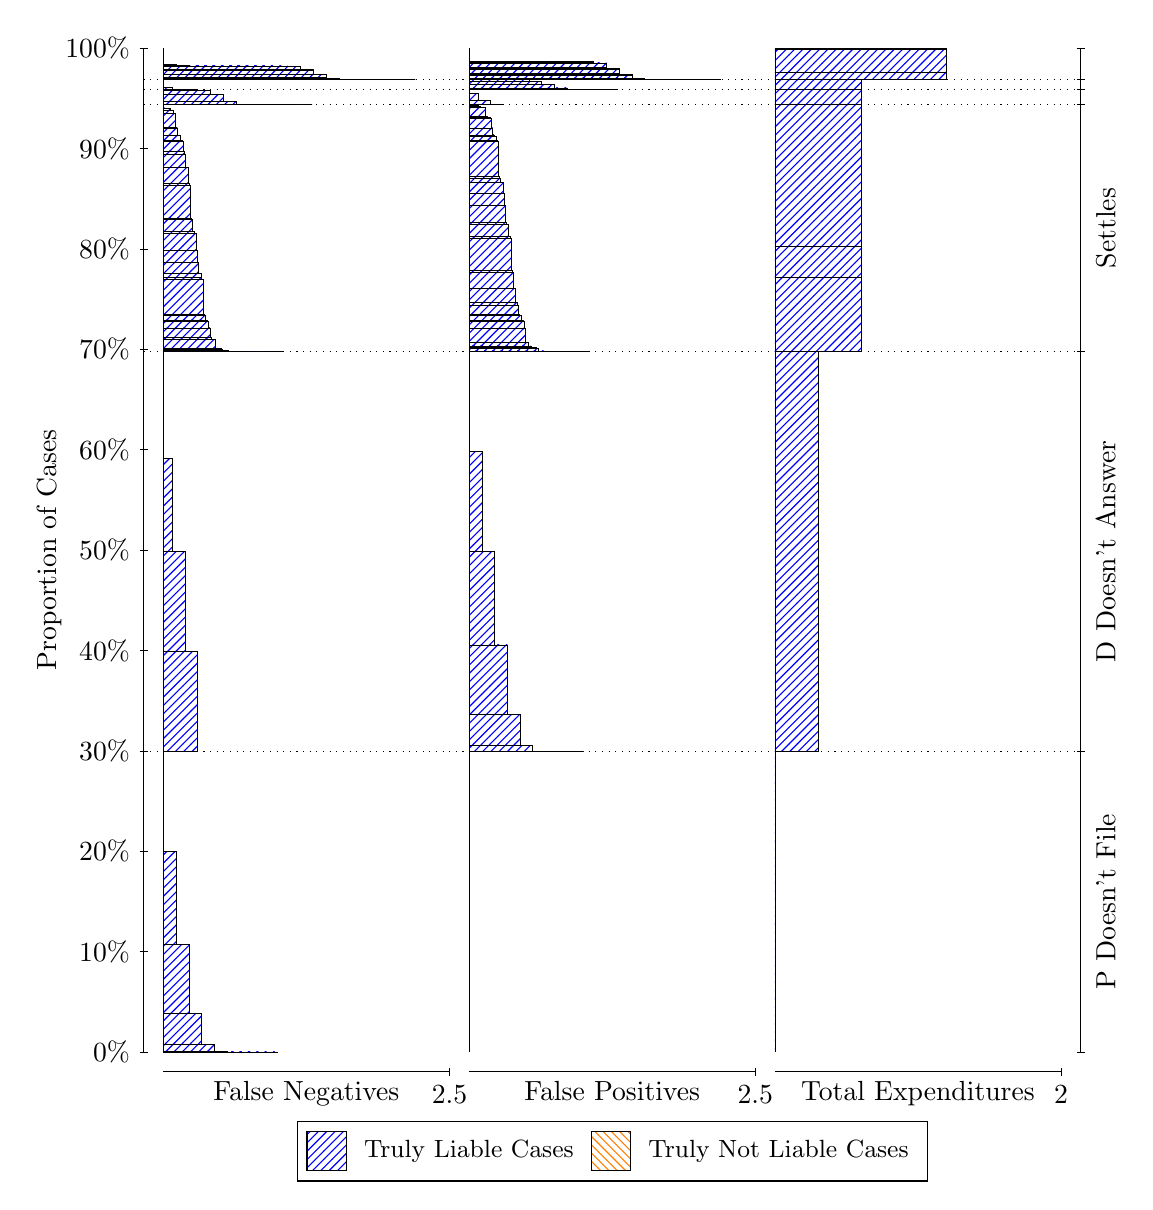
\begin{tikzpicture}
\draw[black, very thin] (1.5,1.75) -- (1.5,14.5);
\node[rotate=90, text=black, anchor=center] at (0.3, 8.125) {Proportion of Cases};
\draw[black, very thin] (1.45,1.75) -- (1.55,1.75);
\node[text=black, anchor=east] at (1.45, 1.75) {0\%};
\draw[black, very thin] (1.45,3.025) -- (1.55,3.025);
\node[text=black, anchor=east] at (1.45, 3.025) {10\%};
\draw[black, very thin] (1.45,4.3) -- (1.55,4.3);
\node[text=black, anchor=east] at (1.45, 4.3) {20\%};
\draw[black, very thin] (1.45,5.575) -- (1.55,5.575);
\node[text=black, anchor=east] at (1.45, 5.575) {30\%};
\draw[black, very thin] (1.45,6.85) -- (1.55,6.85);
\node[text=black, anchor=east] at (1.45, 6.85) {40\%};
\draw[black, very thin] (1.45,8.125) -- (1.55,8.125);
\node[text=black, anchor=east] at (1.45, 8.125) {50\%};
\draw[black, very thin] (1.45,9.4) -- (1.55,9.4);
\node[text=black, anchor=east] at (1.45, 9.4) {60\%};
\draw[black, very thin] (1.45,10.675) -- (1.55,10.675);
\node[text=black, anchor=east] at (1.45, 10.675) {70\%};
\draw[black, very thin] (1.45,11.95) -- (1.55,11.95);
\node[text=black, anchor=east] at (1.45, 11.95) {80\%};
\draw[black, very thin] (1.45,13.225) -- (1.55,13.225);
\node[text=black, anchor=east] at (1.45, 13.225) {90\%};
\draw[black, very thin] (1.45,14.5) -- (1.55,14.5);
\node[text=black, anchor=east] at (1.45, 14.5) {100\%};

\draw[black, very thin] (13.4,1.75) -- (13.4,14.5);
\draw[black, very thin] (13.35,1.75) -- (13.45,1.75);
\node[anchor=west] at (13.35, 1.75) {};
\draw[black, very thin] (13.35,5.563) -- (13.45,5.563);
\node[anchor=west] at (13.35, 5.563) {};
\draw[black, very thin] (13.35,10.651) -- (13.45,10.651);
\node[anchor=west] at (13.35, 10.651) {};
\draw[black, very thin] (13.35,13.78) -- (13.45,13.78);
\node[anchor=west] at (13.35, 13.78) {};
\draw[black, very thin] (13.35,13.972) -- (13.45,13.972);
\node[anchor=west] at (13.35, 13.972) {};
\draw[black, very thin] (13.35,14.101) -- (13.45,14.101);
\node[anchor=west] at (13.35, 14.101) {};
\draw[black, very thin] (13.35,14.5) -- (13.45,14.5);
\node[anchor=west] at (13.35, 14.5) {};

\draw[black, very thin, pattern color=blue, pattern=north east lines] (1.75,1.75) rectangle (3.2033,1.75);
\draw[black, very thin, pattern color=blue, pattern=north east lines] (1.75,1.75) rectangle (3.0419,1.75);
\draw[black, very thin, pattern color=blue, pattern=north east lines] (1.75,1.75) rectangle (2.8804,1.75);
\draw[black, very thin, pattern color=blue, pattern=north east lines] (1.75,1.75) rectangle (2.7189,1.7503);
\draw[black, very thin, pattern color=blue, pattern=north east lines] (1.75,1.7503) rectangle (2.5574,1.7582);
\draw[black, very thin, pattern color=blue, pattern=north east lines] (1.75,1.7582) rectangle (2.3959,1.8434);
\draw[black, very thin, pattern color=blue, pattern=north east lines] (1.75,1.8434) rectangle (2.2344,2.2366);
\draw[black, very thin, pattern color=blue, pattern=north east lines] (1.75,2.2366) rectangle (2.073,3.1157);
\draw[black, very thin, pattern color=blue, pattern=north east lines] (1.75,3.1157) rectangle (1.9115,4.2995);
\draw[black, very thin, pattern color=orange, pattern=north west lines] (1.75,4.2995) rectangle (1.75,4.2995);
\draw[black, very thin, pattern color=blue, pattern=north east lines] (1.75,4.2995) rectangle (1.75,5.563);
\draw[black, very thin, pattern color=blue, pattern=north east lines] (1.75,5.563) rectangle (2.186,6.8376);
\draw[black, very thin, pattern color=blue, pattern=north east lines] (1.75,6.8376) rectangle (2.0245,8.1041);
\draw[black, very thin, pattern color=blue, pattern=north east lines] (1.75,8.1041) rectangle (1.863,9.2934);
\draw[black, very thin, pattern color=orange, pattern=north west lines] (1.75,9.2934) rectangle (1.75,9.2934);
\draw[black, very thin, pattern color=blue, pattern=north east lines] (1.75,9.2934) rectangle (1.75,10.651);
\draw[black, very thin, pattern color=blue, pattern=north east lines] (1.75,10.651) rectangle (3.276,10.651);
\draw[black, very thin, pattern color=blue, pattern=north east lines] (1.75,10.651) rectangle (3.2033,10.651);
\draw[black, very thin, pattern color=blue, pattern=north east lines] (1.75,10.651) rectangle (3.1307,10.651);
\draw[black, very thin, pattern color=blue, pattern=north east lines] (1.75,10.651) rectangle (3.1145,10.651);
\draw[black, very thin, pattern color=blue, pattern=north east lines] (1.75,10.651) rectangle (3.058,10.651);
\draw[black, very thin, pattern color=blue, pattern=north east lines] (1.75,10.651) rectangle (3.0419,10.651);
\draw[black, very thin, pattern color=blue, pattern=north east lines] (1.75,10.651) rectangle (2.9853,10.651);
\draw[black, very thin, pattern color=blue, pattern=north east lines] (1.75,10.651) rectangle (2.9692,10.651);
\draw[black, very thin, pattern color=blue, pattern=north east lines] (1.75,10.651) rectangle (2.953,10.651);
\draw[black, very thin, pattern color=blue, pattern=north east lines] (1.75,10.651) rectangle (2.9127,10.651);
\draw[black, very thin, pattern color=blue, pattern=north east lines] (1.75,10.651) rectangle (2.8965,10.651);
\draw[black, very thin, pattern color=blue, pattern=north east lines] (1.75,10.651) rectangle (2.8804,10.651);
\draw[black, very thin, pattern color=blue, pattern=north east lines] (1.75,10.651) rectangle (2.84,10.651);
\draw[black, very thin, pattern color=blue, pattern=north east lines] (1.75,10.651) rectangle (2.8239,10.651);
\draw[black, very thin, pattern color=blue, pattern=north east lines] (1.75,10.651) rectangle (2.8077,10.651);
\draw[black, very thin, pattern color=blue, pattern=north east lines] (1.75,10.651) rectangle (2.7916,10.651);
\draw[black, very thin, pattern color=blue, pattern=north east lines] (1.75,10.651) rectangle (2.7673,10.651);
\draw[black, very thin, pattern color=blue, pattern=north east lines] (1.75,10.651) rectangle (2.7512,10.651);
\draw[black, very thin, pattern color=blue, pattern=north east lines] (1.75,10.651) rectangle (2.735,10.651);
\draw[black, very thin, pattern color=blue, pattern=north east lines] (1.75,10.651) rectangle (2.7189,10.651);
\draw[black, very thin, pattern color=blue, pattern=north east lines] (1.75,10.651) rectangle (2.6785,10.651);
\draw[black, very thin, pattern color=blue, pattern=north east lines] (1.75,10.651) rectangle (2.6624,10.651);
\draw[black, very thin, pattern color=blue, pattern=north east lines] (1.75,10.651) rectangle (2.6462,10.651);
\draw[black, very thin, pattern color=blue, pattern=north east lines] (1.75,10.651) rectangle (2.6301,10.651);
\draw[black, very thin, pattern color=blue, pattern=north east lines] (1.75,10.651) rectangle (2.6059,10.651);
\draw[black, very thin, pattern color=blue, pattern=north east lines] (1.75,10.651) rectangle (2.5897,10.651);
\draw[black, very thin, pattern color=blue, pattern=north east lines] (1.75,10.651) rectangle (2.5736,10.657);
\draw[black, very thin, pattern color=blue, pattern=north east lines] (1.75,10.657) rectangle (2.5574,10.657);
\draw[black, very thin, pattern color=blue, pattern=north east lines] (1.75,10.657) rectangle (2.5493,10.657);
\draw[black, very thin, pattern color=blue, pattern=north east lines] (1.75,10.657) rectangle (2.517,10.658);
\draw[black, very thin, pattern color=blue, pattern=north east lines] (1.75,10.658) rectangle (2.5009,10.674);
\draw[black, very thin, pattern color=blue, pattern=north east lines] (1.75,10.674) rectangle (2.4847,10.682);
\draw[black, very thin, pattern color=blue, pattern=north east lines] (1.75,10.682) rectangle (2.4686,10.684);
\draw[black, very thin, pattern color=blue, pattern=north east lines] (1.75,10.684) rectangle (2.4444,10.688);
\draw[black, very thin, pattern color=blue, pattern=north east lines] (1.75,10.688) rectangle (2.4282,10.688);
\draw[black, very thin, pattern color=blue, pattern=north east lines] (1.75,10.688) rectangle (2.4121,10.798);
\draw[black, very thin, pattern color=blue, pattern=north east lines] (1.75,10.798) rectangle (2.3959,10.802);
\draw[black, very thin, pattern color=blue, pattern=north east lines] (1.75,10.802) rectangle (2.3879,10.805);
\draw[black, very thin, pattern color=blue, pattern=north east lines] (1.75,10.805) rectangle (2.3556,10.825);
\draw[black, very thin, pattern color=blue, pattern=north east lines] (1.75,10.825) rectangle (2.3394,10.945);
\draw[black, very thin, pattern color=blue, pattern=north east lines] (1.75,10.945) rectangle (2.3233,11.032);
\draw[black, very thin, pattern color=blue, pattern=north east lines] (1.75,11.032) rectangle (2.3071,11.047);
\draw[black, very thin, pattern color=blue, pattern=north east lines] (1.75,11.047) rectangle (2.2829,11.107);
\draw[black, very thin, pattern color=blue, pattern=north east lines] (1.75,11.107) rectangle (2.2667,11.115);
\draw[black, very thin, pattern color=blue, pattern=north east lines] (1.75,11.115) rectangle (2.2506,11.56);
\draw[black, very thin, pattern color=blue, pattern=north east lines] (1.75,11.56) rectangle (2.2344,11.586);
\draw[black, very thin, pattern color=blue, pattern=north east lines] (1.75,11.586) rectangle (2.2264,11.634);
\draw[black, very thin, pattern color=blue, pattern=north east lines] (1.75,11.634) rectangle (2.1941,11.773);
\draw[black, very thin, pattern color=blue, pattern=north east lines] (1.75,11.773) rectangle (2.1779,11.929);
\draw[black, very thin, pattern color=blue, pattern=north east lines] (1.75,11.929) rectangle (2.1618,12.143);
\draw[black, very thin, pattern color=blue, pattern=north east lines] (1.75,12.143) rectangle (2.1456,12.17);
\draw[black, very thin, pattern color=blue, pattern=north east lines] (1.75,12.17) rectangle (2.1214,12.321);
\draw[black, very thin, pattern color=blue, pattern=north east lines] (1.75,12.321) rectangle (2.1053,12.342);
\draw[black, very thin, pattern color=blue, pattern=north east lines] (1.75,12.342) rectangle (2.0891,12.756);
\draw[black, very thin, pattern color=blue, pattern=north east lines] (1.75,12.756) rectangle (2.073,12.782);
\draw[black, very thin, pattern color=blue, pattern=north east lines] (1.75,12.782) rectangle (2.0649,12.984);
\draw[black, very thin, pattern color=blue, pattern=north east lines] (1.75,12.984) rectangle (2.0326,13.156);
\draw[black, very thin, pattern color=blue, pattern=north east lines] (1.75,13.156) rectangle (2.0164,13.195);
\draw[black, very thin, pattern color=blue, pattern=north east lines] (1.75,13.195) rectangle (2.0003,13.316);
\draw[black, very thin, pattern color=blue, pattern=north east lines] (1.75,13.316) rectangle (1.9841,13.326);
\draw[black, very thin, pattern color=blue, pattern=north east lines] (1.75,13.326) rectangle (1.9599,13.387);
\draw[black, very thin, pattern color=blue, pattern=north east lines] (1.75,13.387) rectangle (1.9438,13.395);
\draw[black, very thin, pattern color=blue, pattern=north east lines] (1.75,13.395) rectangle (1.9276,13.487);
\draw[black, very thin, pattern color=blue, pattern=north east lines] (1.75,13.487) rectangle (1.9115,13.492);
\draw[black, very thin, pattern color=blue, pattern=north east lines] (1.75,13.492) rectangle (1.9034,13.673);
\draw[black, very thin, pattern color=blue, pattern=north east lines] (1.75,13.673) rectangle (1.8711,13.713);
\draw[black, very thin, pattern color=blue, pattern=north east lines] (1.75,13.713) rectangle (1.855,13.715);
\draw[black, very thin, pattern color=blue, pattern=north east lines] (1.75,13.715) rectangle (1.8388,13.731);
\draw[black, very thin, pattern color=blue, pattern=north east lines] (1.75,13.731) rectangle (1.8227,13.732);
\draw[black, very thin, pattern color=blue, pattern=north east lines] (1.75,13.732) rectangle (1.7984,13.736);
\draw[black, very thin, pattern color=blue, pattern=north east lines] (1.75,13.736) rectangle (1.7823,13.736);
\draw[black, very thin, pattern color=blue, pattern=north east lines] (1.75,13.736) rectangle (1.7661,13.741);
\draw[black, very thin, pattern color=orange, pattern=north west lines] (1.75,13.741) rectangle (1.75,13.741);
\draw[black, very thin, pattern color=blue, pattern=north east lines] (1.75,13.741) rectangle (1.75,13.78);
\draw[black, very thin, pattern color=blue, pattern=north east lines] (1.75,13.78) rectangle (3.6393,13.78);
\draw[black, very thin, pattern color=blue, pattern=north east lines] (1.75,13.78) rectangle (3.4779,13.78);
\draw[black, very thin, pattern color=blue, pattern=north east lines] (1.75,13.78) rectangle (3.3164,13.78);
\draw[black, very thin, pattern color=blue, pattern=north east lines] (1.75,13.78) rectangle (3.1549,13.78);
\draw[black, very thin, pattern color=blue, pattern=north east lines] (1.75,13.78) rectangle (2.9934,13.78);
\draw[black, very thin, pattern color=blue, pattern=north east lines] (1.75,13.78) rectangle (2.8319,13.784);
\draw[black, very thin, pattern color=blue, pattern=north east lines] (1.75,13.784) rectangle (2.6704,13.824);
\draw[black, very thin, pattern color=blue, pattern=north east lines] (1.75,13.824) rectangle (2.509,13.914);
\draw[black, very thin, pattern color=blue, pattern=north east lines] (1.75,13.914) rectangle (2.3475,13.963);
\draw[black, very thin, pattern color=blue, pattern=north east lines] (1.75,13.963) rectangle (2.186,13.972);
\draw[black, very thin, pattern color=orange, pattern=north west lines] (1.75,13.972) rectangle (1.75,13.972);
\draw[black, very thin, pattern color=blue, pattern=north east lines] (1.75,13.972) rectangle (2.186,13.973);
\draw[black, very thin, pattern color=blue, pattern=north east lines] (1.75,13.973) rectangle (2.0245,13.977);
\draw[black, very thin, pattern color=blue, pattern=north east lines] (1.75,13.977) rectangle (1.863,13.997);
\draw[black, very thin, pattern color=orange, pattern=north west lines] (1.75,13.997) rectangle (1.75,13.997);
\draw[black, very thin, pattern color=blue, pattern=north east lines] (1.75,13.997) rectangle (1.75,14.101);
\draw[black, very thin, pattern color=blue, pattern=north east lines] (1.75,14.101) rectangle (4.9473,14.101);
\draw[black, very thin, pattern color=blue, pattern=north east lines] (1.75,14.101) rectangle (4.7859,14.101);
\draw[black, very thin, pattern color=blue, pattern=north east lines] (1.75,14.101) rectangle (4.6244,14.101);
\draw[black, very thin, pattern color=blue, pattern=north east lines] (1.75,14.101) rectangle (4.6244,14.101);
\draw[black, very thin, pattern color=blue, pattern=north east lines] (1.75,14.101) rectangle (4.4629,14.101);
\draw[black, very thin, pattern color=blue, pattern=north east lines] (1.75,14.101) rectangle (4.3014,14.101);
\draw[black, very thin, pattern color=blue, pattern=north east lines] (1.75,14.101) rectangle (4.1399,14.104);
\draw[black, very thin, pattern color=blue, pattern=north east lines] (1.75,14.104) rectangle (3.9784,14.118);
\draw[black, very thin, pattern color=blue, pattern=north east lines] (1.75,14.118) rectangle (3.817,14.13);
\draw[black, very thin, pattern color=blue, pattern=north east lines] (1.75,14.13) rectangle (3.817,14.161);
\draw[black, very thin, pattern color=blue, pattern=north east lines] (1.75,14.161) rectangle (3.6555,14.221);
\draw[black, very thin, pattern color=blue, pattern=north east lines] (1.75,14.221) rectangle (3.6555,14.23);
\draw[black, very thin, pattern color=blue, pattern=north east lines] (1.75,14.23) rectangle (3.494,14.269);
\draw[black, very thin, pattern color=blue, pattern=north east lines] (1.75,14.269) rectangle (3.3325,14.27);
\draw[black, very thin, pattern color=blue, pattern=north east lines] (1.75,14.27) rectangle (3.3325,14.274);
\draw[black, very thin, pattern color=blue, pattern=north east lines] (1.75,14.274) rectangle (3.171,14.274);
\draw[black, very thin, pattern color=blue, pattern=north east lines] (1.75,14.274) rectangle (3.171,14.274);
\draw[black, very thin, pattern color=blue, pattern=north east lines] (1.75,14.274) rectangle (3.171,14.274);
\draw[black, very thin, pattern color=blue, pattern=north east lines] (1.75,14.274) rectangle (3.0096,14.274);
\draw[black, very thin, pattern color=blue, pattern=north east lines] (1.75,14.274) rectangle (3.0096,14.274);
\draw[black, very thin, pattern color=blue, pattern=north east lines] (1.75,14.274) rectangle (2.8804,14.274);
\draw[black, very thin, pattern color=blue, pattern=north east lines] (1.75,14.274) rectangle (2.8481,14.274);
\draw[black, very thin, pattern color=blue, pattern=north east lines] (1.75,14.274) rectangle (2.7189,14.274);
\draw[black, very thin, pattern color=blue, pattern=north east lines] (1.75,14.274) rectangle (2.7189,14.274);
\draw[black, very thin, pattern color=blue, pattern=north east lines] (1.75,14.274) rectangle (2.6866,14.274);
\draw[black, very thin, pattern color=blue, pattern=north east lines] (1.75,14.274) rectangle (2.5574,14.274);
\draw[black, very thin, pattern color=blue, pattern=north east lines] (1.75,14.274) rectangle (2.5251,14.274);
\draw[black, very thin, pattern color=blue, pattern=north east lines] (1.75,14.274) rectangle (2.3959,14.274);
\draw[black, very thin, pattern color=blue, pattern=north east lines] (1.75,14.274) rectangle (2.3959,14.274);
\draw[black, very thin, pattern color=blue, pattern=north east lines] (1.75,14.274) rectangle (2.2344,14.274);
\draw[black, very thin, pattern color=blue, pattern=north east lines] (1.75,14.274) rectangle (2.2344,14.274);
\draw[black, very thin, pattern color=blue, pattern=north east lines] (1.75,14.274) rectangle (2.2344,14.274);
\draw[black, very thin, pattern color=blue, pattern=north east lines] (1.75,14.274) rectangle (2.073,14.274);
\draw[black, very thin, pattern color=blue, pattern=north east lines] (1.75,14.274) rectangle (2.073,14.275);
\draw[black, very thin, pattern color=blue, pattern=north east lines] (1.75,14.275) rectangle (1.9115,14.277);
\draw[black, very thin, pattern color=blue, pattern=north east lines] (1.75,14.277) rectangle (1.9115,14.281);
\draw[black, very thin, pattern color=blue, pattern=north east lines] (1.75,14.281) rectangle (1.9115,14.29);
\draw[black, very thin, pattern color=orange, pattern=north west lines] (1.75,14.29) rectangle (1.75,14.29);
\draw[black, very thin, pattern color=blue, pattern=north east lines] (1.75,14.29) rectangle (1.75,14.5);
\draw[black, very thin, pattern color=orange, pattern=north west lines] (5.6333,1.75) rectangle (5.6333,1.75);
\draw[black, very thin, pattern color=blue, pattern=north east lines] (5.6333,1.75) rectangle (5.6333,5.563);
\draw[black, very thin, pattern color=orange, pattern=north west lines] (5.6333,5.563) rectangle (7.0867,5.563);
\draw[black, very thin, pattern color=blue, pattern=north east lines] (5.6333,5.563) rectangle (7.0867,5.563);
\draw[black, very thin, pattern color=blue, pattern=north east lines] (5.6333,5.563) rectangle (6.9252,5.563);
\draw[black, very thin, pattern color=blue, pattern=north east lines] (5.6333,5.563) rectangle (6.7637,5.5631);
\draw[black, very thin, pattern color=blue, pattern=north east lines] (5.6333,5.5631) rectangle (6.6022,5.5686);
\draw[black, very thin, pattern color=blue, pattern=north east lines] (5.6333,5.5686) rectangle (6.4407,5.6481);
\draw[black, very thin, pattern color=blue, pattern=north east lines] (5.6333,5.6481) rectangle (6.2793,6.039);
\draw[black, very thin, pattern color=blue, pattern=north east lines] (5.6333,6.039) rectangle (6.1178,6.9203);
\draw[black, very thin, pattern color=blue, pattern=north east lines] (5.6333,6.9203) rectangle (5.9563,8.1096);
\draw[black, very thin, pattern color=blue, pattern=north east lines] (5.6333,8.1096) rectangle (5.7948,9.3761);
\draw[black, very thin, pattern color=blue, pattern=north east lines] (5.6333,9.3761) rectangle (5.6333,10.651);
\draw[black, very thin, pattern color=orange, pattern=north west lines] (5.6333,10.651) rectangle (7.1593,10.651);
\draw[black, very thin, pattern color=blue, pattern=north east lines] (5.6333,10.651) rectangle (7.1593,10.651);
\draw[black, very thin, pattern color=blue, pattern=north east lines] (5.6333,10.651) rectangle (6.9979,10.651);
\draw[black, very thin, pattern color=orange, pattern=north west lines] (5.6333,10.651) rectangle (6.9413,10.651);
\draw[black, very thin, pattern color=blue, pattern=north east lines] (5.6333,10.651) rectangle (6.9413,10.651);
\draw[black, very thin, pattern color=orange, pattern=north west lines] (5.6333,10.651) rectangle (6.8687,10.651);
\draw[black, very thin, pattern color=blue, pattern=north east lines] (5.6333,10.651) rectangle (6.8687,10.651);
\draw[black, very thin, pattern color=blue, pattern=north east lines] (5.6333,10.651) rectangle (6.8364,10.651);
\draw[black, very thin, pattern color=orange, pattern=north west lines] (5.6333,10.651) rectangle (6.796,10.651);
\draw[black, very thin, pattern color=blue, pattern=north east lines] (5.6333,10.651) rectangle (6.796,10.651);
\draw[black, very thin, pattern color=blue, pattern=north east lines] (5.6333,10.651) rectangle (6.7799,10.651);
\draw[black, very thin, pattern color=orange, pattern=north west lines] (5.6333,10.651) rectangle (6.7233,10.651);
\draw[black, very thin, pattern color=blue, pattern=north east lines] (5.6333,10.651) rectangle (6.7233,10.651);
\draw[black, very thin, pattern color=blue, pattern=north east lines] (5.6333,10.651) rectangle (6.7072,10.651);
\draw[black, very thin, pattern color=blue, pattern=north east lines] (5.6333,10.651) rectangle (6.6749,10.652);
\draw[black, very thin, pattern color=orange, pattern=north west lines] (5.6333,10.652) rectangle (6.6507,10.652);
\draw[black, very thin, pattern color=blue, pattern=north east lines] (5.6333,10.652) rectangle (6.6507,10.652);
\draw[black, very thin, pattern color=blue, pattern=north east lines] (5.6333,10.652) rectangle (6.6345,10.652);
\draw[black, very thin, pattern color=blue, pattern=north east lines] (5.6333,10.652) rectangle (6.6184,10.652);
\draw[black, very thin, pattern color=orange, pattern=north west lines] (5.6333,10.652) rectangle (6.578,10.652);
\draw[black, very thin, pattern color=blue, pattern=north east lines] (5.6333,10.652) rectangle (6.578,10.653);
\draw[black, very thin, pattern color=blue, pattern=north east lines] (5.6333,10.653) rectangle (6.5619,10.653);
\draw[black, very thin, pattern color=blue, pattern=north east lines] (5.6333,10.653) rectangle (6.5457,10.655);
\draw[black, very thin, pattern color=blue, pattern=north east lines] (5.6333,10.655) rectangle (6.5134,10.689);
\draw[black, very thin, pattern color=orange, pattern=north west lines] (5.6333,10.689) rectangle (6.5053,10.689);
\draw[black, very thin, pattern color=blue, pattern=north east lines] (5.6333,10.689) rectangle (6.5053,10.689);
\draw[black, very thin, pattern color=blue, pattern=north east lines] (5.6333,10.689) rectangle (6.4892,10.694);
\draw[black, very thin, pattern color=blue, pattern=north east lines] (5.6333,10.694) rectangle (6.473,10.695);
\draw[black, very thin, pattern color=blue, pattern=north east lines] (5.6333,10.695) rectangle (6.4569,10.699);
\draw[black, very thin, pattern color=orange, pattern=north west lines] (5.6333,10.699) rectangle (6.4327,10.699);
\draw[black, very thin, pattern color=blue, pattern=north east lines] (5.6333,10.699) rectangle (6.4327,10.7);
\draw[black, very thin, pattern color=blue, pattern=north east lines] (5.6333,10.7) rectangle (6.4165,10.716);
\draw[black, very thin, pattern color=blue, pattern=north east lines] (5.6333,10.716) rectangle (6.4004,10.718);
\draw[black, very thin, pattern color=blue, pattern=north east lines] (5.6333,10.718) rectangle (6.3842,10.758);
\draw[black, very thin, pattern color=blue, pattern=north east lines] (5.6333,10.758) rectangle (6.3519,10.939);
\draw[black, very thin, pattern color=blue, pattern=north east lines] (5.6333,10.939) rectangle (6.3439,10.944);
\draw[black, very thin, pattern color=blue, pattern=north east lines] (5.6333,10.944) rectangle (6.3277,11.036);
\draw[black, very thin, pattern color=blue, pattern=north east lines] (5.6333,11.036) rectangle (6.3116,11.044);
\draw[black, very thin, pattern color=blue, pattern=north east lines] (5.6333,11.044) rectangle (6.2954,11.104);
\draw[black, very thin, pattern color=blue, pattern=north east lines] (5.6333,11.104) rectangle (6.2712,11.115);
\draw[black, very thin, pattern color=blue, pattern=north east lines] (5.6333,11.115) rectangle (6.255,11.235);
\draw[black, very thin, pattern color=blue, pattern=north east lines] (5.6333,11.235) rectangle (6.2389,11.274);
\draw[black, very thin, pattern color=blue, pattern=north east lines] (5.6333,11.274) rectangle (6.2227,11.446);
\draw[black, very thin, pattern color=blue, pattern=north east lines] (5.6333,11.446) rectangle (6.1904,11.648);
\draw[black, very thin, pattern color=blue, pattern=north east lines] (5.6333,11.648) rectangle (6.1824,11.675);
\draw[black, very thin, pattern color=blue, pattern=north east lines] (5.6333,11.675) rectangle (6.1662,12.089);
\draw[black, very thin, pattern color=blue, pattern=north east lines] (5.6333,12.089) rectangle (6.1501,12.109);
\draw[black, very thin, pattern color=blue, pattern=north east lines] (5.6333,12.109) rectangle (6.1339,12.261);
\draw[black, very thin, pattern color=blue, pattern=north east lines] (5.6333,12.261) rectangle (6.1097,12.288);
\draw[black, very thin, pattern color=blue, pattern=north east lines] (5.6333,12.288) rectangle (6.0936,12.501);
\draw[black, very thin, pattern color=blue, pattern=north east lines] (5.6333,12.501) rectangle (6.0774,12.657);
\draw[black, very thin, pattern color=blue, pattern=north east lines] (5.6333,12.657) rectangle (6.0613,12.797);
\draw[black, very thin, pattern color=blue, pattern=north east lines] (5.6333,12.797) rectangle (6.029,12.845);
\draw[black, very thin, pattern color=blue, pattern=north east lines] (5.6333,12.845) rectangle (6.0209,12.871);
\draw[black, very thin, pattern color=blue, pattern=north east lines] (5.6333,12.871) rectangle (6.0047,13.315);
\draw[black, very thin, pattern color=blue, pattern=north east lines] (5.6333,13.315) rectangle (5.9886,13.324);
\draw[black, very thin, pattern color=blue, pattern=north east lines] (5.6333,13.324) rectangle (5.9724,13.384);
\draw[black, very thin, pattern color=blue, pattern=north east lines] (5.6333,13.384) rectangle (5.9482,13.398);
\draw[black, very thin, pattern color=blue, pattern=north east lines] (5.6333,13.398) rectangle (5.9321,13.486);
\draw[black, very thin, pattern color=blue, pattern=north east lines] (5.6333,13.486) rectangle (5.9159,13.606);
\draw[black, very thin, pattern color=blue, pattern=north east lines] (5.6333,13.606) rectangle (5.8998,13.626);
\draw[black, very thin, pattern color=blue, pattern=north east lines] (5.6333,13.626) rectangle (5.8675,13.628);
\draw[black, very thin, pattern color=blue, pattern=north east lines] (5.6333,13.628) rectangle (5.8594,13.632);
\draw[black, very thin, pattern color=blue, pattern=north east lines] (5.6333,13.632) rectangle (5.8433,13.742);
\draw[black, very thin, pattern color=blue, pattern=north east lines] (5.6333,13.742) rectangle (5.8271,13.743);
\draw[black, very thin, pattern color=blue, pattern=north east lines] (5.6333,13.743) rectangle (5.811,13.747);
\draw[black, very thin, pattern color=blue, pattern=north east lines] (5.6333,13.747) rectangle (5.7867,13.748);
\draw[black, very thin, pattern color=blue, pattern=north east lines] (5.6333,13.748) rectangle (5.7706,13.756);
\draw[black, very thin, pattern color=blue, pattern=north east lines] (5.6333,13.756) rectangle (5.7544,13.773);
\draw[black, very thin, pattern color=blue, pattern=north east lines] (5.6333,13.773) rectangle (5.7383,13.774);
\draw[black, very thin, pattern color=blue, pattern=north east lines] (5.6333,13.774) rectangle (5.706,13.774);
\draw[black, very thin, pattern color=blue, pattern=north east lines] (5.6333,13.774) rectangle (5.6979,13.774);
\draw[black, very thin, pattern color=blue, pattern=north east lines] (5.6333,13.774) rectangle (5.6818,13.779);
\draw[black, very thin, pattern color=blue, pattern=north east lines] (5.6333,13.779) rectangle (5.6656,13.779);
\draw[black, very thin, pattern color=blue, pattern=north east lines] (5.6333,13.779) rectangle (5.6495,13.779);
\draw[black, very thin, pattern color=blue, pattern=north east lines] (5.6333,13.779) rectangle (5.6333,13.78);
\draw[black, very thin, pattern color=orange, pattern=north west lines] (5.6333,13.78) rectangle (6.0693,13.78);
\draw[black, very thin, pattern color=blue, pattern=north east lines] (5.6333,13.78) rectangle (6.0693,13.789);
\draw[black, very thin, pattern color=blue, pattern=north east lines] (5.6333,13.789) rectangle (5.9079,13.838);
\draw[black, very thin, pattern color=blue, pattern=north east lines] (5.6333,13.838) rectangle (5.7464,13.928);
\draw[black, very thin, pattern color=blue, pattern=north east lines] (5.6333,13.928) rectangle (5.6333,13.972);
\draw[black, very thin, pattern color=orange, pattern=north west lines] (5.6333,13.972) rectangle (7.5227,13.972);
\draw[black, very thin, pattern color=blue, pattern=north east lines] (5.6333,13.972) rectangle (7.5227,13.972);
\draw[black, very thin, pattern color=blue, pattern=north east lines] (5.6333,13.972) rectangle (7.3612,13.972);
\draw[black, very thin, pattern color=blue, pattern=north east lines] (5.6333,13.972) rectangle (7.1997,13.972);
\draw[black, very thin, pattern color=blue, pattern=north east lines] (5.6333,13.972) rectangle (7.0382,13.974);
\draw[black, very thin, pattern color=blue, pattern=north east lines] (5.6333,13.974) rectangle (6.8767,13.994);
\draw[black, very thin, pattern color=blue, pattern=north east lines] (5.6333,13.994) rectangle (6.7153,14.039);
\draw[black, very thin, pattern color=blue, pattern=north east lines] (5.6333,14.039) rectangle (6.5538,14.077);
\draw[black, very thin, pattern color=blue, pattern=north east lines] (5.6333,14.077) rectangle (6.3923,14.097);
\draw[black, very thin, pattern color=blue, pattern=north east lines] (5.6333,14.097) rectangle (6.2308,14.101);
\draw[black, very thin, pattern color=blue, pattern=north east lines] (5.6333,14.101) rectangle (6.0693,14.101);
\draw[black, very thin, pattern color=orange, pattern=north west lines] (5.6333,14.101) rectangle (8.8307,14.101);
\draw[black, very thin, pattern color=blue, pattern=north east lines] (5.6333,14.101) rectangle (8.8307,14.101);
\draw[black, very thin, pattern color=blue, pattern=north east lines] (5.6333,14.101) rectangle (8.6692,14.101);
\draw[black, very thin, pattern color=orange, pattern=north west lines] (5.6333,14.101) rectangle (8.6692,14.101);
\draw[black, very thin, pattern color=blue, pattern=north east lines] (5.6333,14.101) rectangle (8.6692,14.101);
\draw[black, very thin, pattern color=orange, pattern=north west lines] (5.6333,14.101) rectangle (8.5077,14.101);
\draw[black, very thin, pattern color=blue, pattern=north east lines] (5.6333,14.101) rectangle (8.5077,14.101);
\draw[black, very thin, pattern color=blue, pattern=north east lines] (5.6333,14.101) rectangle (8.5077,14.101);
\draw[black, very thin, pattern color=blue, pattern=north east lines] (5.6333,14.101) rectangle (8.3462,14.101);
\draw[black, very thin, pattern color=orange, pattern=north west lines] (5.6333,14.101) rectangle (8.3462,14.101);
\draw[black, very thin, pattern color=blue, pattern=north east lines] (5.6333,14.101) rectangle (8.3462,14.101);
\draw[black, very thin, pattern color=blue, pattern=north east lines] (5.6333,14.101) rectangle (8.3462,14.101);
\draw[black, very thin, pattern color=blue, pattern=north east lines] (5.6333,14.101) rectangle (8.1847,14.101);
\draw[black, very thin, pattern color=orange, pattern=north west lines] (5.6333,14.101) rectangle (8.1847,14.101);
\draw[black, very thin, pattern color=blue, pattern=north east lines] (5.6333,14.101) rectangle (8.1847,14.101);
\draw[black, very thin, pattern color=blue, pattern=north east lines] (5.6333,14.101) rectangle (8.1847,14.102);
\draw[black, very thin, pattern color=blue, pattern=north east lines] (5.6333,14.102) rectangle (8.0233,14.103);
\draw[black, very thin, pattern color=orange, pattern=north west lines] (5.6333,14.103) rectangle (8.0233,14.103);
\draw[black, very thin, pattern color=blue, pattern=north east lines] (5.6333,14.103) rectangle (8.0233,14.104);
\draw[black, very thin, pattern color=blue, pattern=north east lines] (5.6333,14.104) rectangle (8.0233,14.104);
\draw[black, very thin, pattern color=blue, pattern=north east lines] (5.6333,14.104) rectangle (7.8618,14.106);
\draw[black, very thin, pattern color=blue, pattern=north east lines] (5.6333,14.106) rectangle (7.8618,14.113);
\draw[black, very thin, pattern color=orange, pattern=north west lines] (5.6333,14.113) rectangle (7.8618,14.113);
\draw[black, very thin, pattern color=blue, pattern=north east lines] (5.6333,14.113) rectangle (7.8618,14.115);
\draw[black, very thin, pattern color=blue, pattern=north east lines] (5.6333,14.115) rectangle (7.8618,14.119);
\draw[black, very thin, pattern color=blue, pattern=north east lines] (5.6333,14.119) rectangle (7.7003,14.121);
\draw[black, very thin, pattern color=blue, pattern=north east lines] (5.6333,14.121) rectangle (7.7003,14.153);
\draw[black, very thin, pattern color=orange, pattern=north west lines] (5.6333,14.153) rectangle (7.7003,14.153);
\draw[black, very thin, pattern color=blue, pattern=north east lines] (5.6333,14.153) rectangle (7.7003,14.164);
\draw[black, very thin, pattern color=blue, pattern=north east lines] (5.6333,14.164) rectangle (7.5388,14.175);
\draw[black, very thin, pattern color=blue, pattern=north east lines] (5.6333,14.175) rectangle (7.5388,14.234);
\draw[black, very thin, pattern color=blue, pattern=north east lines] (5.6333,14.234) rectangle (7.5388,14.244);
\draw[black, very thin, pattern color=blue, pattern=north east lines] (5.6333,14.244) rectangle (7.3773,14.259);
\draw[black, very thin, pattern color=blue, pattern=north east lines] (5.6333,14.259) rectangle (7.3773,14.309);
\draw[black, very thin, pattern color=blue, pattern=north east lines] (5.6333,14.309) rectangle (7.3773,14.311);
\draw[black, very thin, pattern color=blue, pattern=north east lines] (5.6333,14.311) rectangle (7.2159,14.322);
\draw[black, very thin, pattern color=blue, pattern=north east lines] (5.6333,14.322) rectangle (7.2159,14.327);
\draw[black, very thin, pattern color=blue, pattern=north east lines] (5.6333,14.327) rectangle (7.2159,14.327);
\draw[black, very thin, pattern color=blue, pattern=north east lines] (5.6333,14.327) rectangle (7.0544,14.327);
\draw[black, very thin, pattern color=blue, pattern=north east lines] (5.6333,14.327) rectangle (7.0544,14.327);
\draw[black, very thin, pattern color=blue, pattern=north east lines] (5.6333,14.327) rectangle (7.0544,14.327);
\draw[black, very thin, pattern color=blue, pattern=north east lines] (5.6333,14.327) rectangle (6.8929,14.327);
\draw[black, very thin, pattern color=blue, pattern=north east lines] (5.6333,14.327) rectangle (6.8929,14.327);
\draw[black, very thin, pattern color=blue, pattern=north east lines] (5.6333,14.327) rectangle (6.8929,14.327);
\draw[black, very thin, pattern color=blue, pattern=north east lines] (5.6333,14.327) rectangle (6.7314,14.327);
\draw[black, very thin, pattern color=blue, pattern=north east lines] (5.6333,14.327) rectangle (6.7314,14.327);
\draw[black, very thin, pattern color=orange, pattern=north west lines] (5.6333,14.327) rectangle (6.6022,14.327);
\draw[black, very thin, pattern color=blue, pattern=north east lines] (5.6333,14.327) rectangle (6.6022,14.327);
\draw[black, very thin, pattern color=blue, pattern=north east lines] (5.6333,14.327) rectangle (6.5699,14.327);
\draw[black, very thin, pattern color=blue, pattern=north east lines] (5.6333,14.327) rectangle (6.5699,14.327);
\draw[black, very thin, pattern color=orange, pattern=north west lines] (5.6333,14.327) rectangle (6.4407,14.327);
\draw[black, very thin, pattern color=blue, pattern=north east lines] (5.6333,14.327) rectangle (6.4407,14.327);
\draw[black, very thin, pattern color=blue, pattern=north east lines] (5.6333,14.327) rectangle (6.4084,14.327);
\draw[black, very thin, pattern color=blue, pattern=north east lines] (5.6333,14.327) rectangle (6.2793,14.327);
\draw[black, very thin, pattern color=orange, pattern=north west lines] (5.6333,14.327) rectangle (6.2793,14.327);
\draw[black, very thin, pattern color=blue, pattern=north east lines] (5.6333,14.327) rectangle (6.2793,14.327);
\draw[black, very thin, pattern color=blue, pattern=north east lines] (5.6333,14.327) rectangle (6.247,14.327);
\draw[black, very thin, pattern color=blue, pattern=north east lines] (5.6333,14.327) rectangle (6.1178,14.327);
\draw[black, very thin, pattern color=orange, pattern=north west lines] (5.6333,14.327) rectangle (6.1178,14.327);
\draw[black, very thin, pattern color=blue, pattern=north east lines] (5.6333,14.327) rectangle (6.1178,14.327);
\draw[black, very thin, pattern color=blue, pattern=north east lines] (5.6333,14.327) rectangle (5.9563,14.327);
\draw[black, very thin, pattern color=orange, pattern=north west lines] (5.6333,14.327) rectangle (5.9563,14.327);
\draw[black, very thin, pattern color=blue, pattern=north east lines] (5.6333,14.327) rectangle (5.9563,14.328);
\draw[black, very thin, pattern color=blue, pattern=north east lines] (5.6333,14.328) rectangle (5.7948,14.328);
\draw[black, very thin, pattern color=orange, pattern=north west lines] (5.6333,14.328) rectangle (5.7948,14.328);
\draw[black, very thin, pattern color=blue, pattern=north east lines] (5.6333,14.328) rectangle (5.7948,14.332);
\draw[black, very thin, pattern color=blue, pattern=north east lines] (5.6333,14.332) rectangle (5.7948,14.332);
\draw[black, very thin, pattern color=orange, pattern=north west lines] (5.6333,14.332) rectangle (5.6333,14.332);
\draw[black, very thin, pattern color=blue, pattern=north east lines] (5.6333,14.332) rectangle (5.6333,14.5);
\draw[black, very thin, pattern color=orange, pattern=north west lines] (9.5167,1.75) rectangle (9.5167,1.75);
\draw[black, very thin, pattern color=blue, pattern=north east lines] (9.5167,1.75) rectangle (9.5167,5.563);
\draw[black, very thin, pattern color=orange, pattern=north west lines] (9.5167,5.563) rectangle (10.062,5.563);
\draw[black, very thin, pattern color=blue, pattern=north east lines] (9.5167,5.563) rectangle (10.062,10.651);
\draw[black, very thin, pattern color=orange, pattern=north west lines] (9.5167,10.651) rectangle (10.607,10.651);
\draw[black, very thin, pattern color=blue, pattern=north east lines] (9.5167,10.651) rectangle (10.607,11.586);
\draw[black, very thin, pattern color=orange, pattern=north west lines] (9.5167,11.586) rectangle (10.607,11.586);
\draw[black, very thin, pattern color=blue, pattern=north east lines] (9.5167,11.586) rectangle (10.607,11.982);
\draw[black, very thin, pattern color=orange, pattern=north west lines] (9.5167,11.982) rectangle (10.607,11.982);
\draw[black, very thin, pattern color=blue, pattern=north east lines] (9.5167,11.982) rectangle (10.607,13.78);
\draw[black, very thin, pattern color=orange, pattern=north west lines] (9.5167,13.78) rectangle (10.607,13.78);
\draw[black, very thin, pattern color=blue, pattern=north east lines] (9.5167,13.78) rectangle (10.607,13.972);
\draw[black, very thin, pattern color=orange, pattern=north west lines] (9.5167,13.972) rectangle (10.607,13.972);
\draw[black, very thin, pattern color=blue, pattern=north east lines] (9.5167,13.972) rectangle (10.607,14.101);
\draw[black, very thin, pattern color=orange, pattern=north west lines] (9.5167,14.101) rectangle (11.697,14.101);
\draw[black, very thin, pattern color=blue, pattern=north east lines] (9.5167,14.101) rectangle (11.697,14.189);
\draw[black, very thin, pattern color=orange, pattern=north west lines] (9.5167,14.189) rectangle (11.697,14.189);
\draw[black, very thin, pattern color=blue, pattern=north east lines] (9.5167,14.189) rectangle (11.697,14.483);
\draw[black, very thin, pattern color=orange, pattern=north west lines] (9.5167,14.483) rectangle (11.697,14.483);
\draw[black, very thin, pattern color=blue, pattern=north east lines] (9.5167,14.483) rectangle (11.697,14.5);
\draw[black, dotted] (1.5,5.563) -- (13.4,5.563);
\draw[black, dotted] (1.5,10.651) -- (13.4,10.651);
\draw[black, dotted] (1.5,13.78) -- (13.4,13.78);
\draw[black, dotted] (1.5,13.972) -- (13.4,13.972);
\draw[black, dotted] (1.5,14.101) -- (13.4,14.101);
\draw[black, very thin] (1.75,1.5) -- (5.3833,1.5);
\node[text=black, anchor=north] at (3.5667, 1.5) {False Negatives};
\draw[black, very thin] (5.3833,1.45) -- (5.3833,1.55);
\node[text=black, anchor=north] at (5.3833, 1.45) {2.5};

\draw[black, very thin] (5.6333,1.5) -- (9.2667,1.5);
\node[text=black, anchor=north] at (7.45, 1.5) {False Positives};
\draw[black, very thin] (9.2667,1.45) -- (9.2667,1.55);
\node[text=black, anchor=north] at (9.2667, 1.45) {2.5};

\draw[black, very thin] (9.5167,1.5) -- (13.15,1.5);
\node[text=black, anchor=north] at (11.333, 1.5) {Total Expenditures};
\draw[black, very thin] (13.15,1.45) -- (13.15,1.55);
\node[text=black, anchor=north] at (13.15, 1.45) {2};

\node[text=black, centered, rotate=90] at (13.72, 3.6565) {P Doesn't File};
\node[text=black, centered, rotate=90] at (13.72, 8.1069) {D Doesn't Answer};
\node[text=black, centered, rotate=90] at (13.72, 12.215) {Settles};




\draw (7.449999999999999,1.5) node[draw=none] (baseCoordinate) {};
\begin{scope}[align=center]
        \matrix[scale=0.5, draw=black, below=0.5cm of baseCoordinate, nodes={draw}, column sep=0.1cm]{
            \node[rectangle, draw, minimum width=0.5cm, minimum height=0.5cm, pattern color=blue, pattern=north east lines] {}; &
            \node[draw=none, font=\small, text=black] (B) {Truly Liable Cases}; &
            \node[rectangle, draw, minimum width=0.5cm, minimum height=0.5cm, pattern color=orange, pattern=north west lines] {}; &
            \node[draw=none, font=\small, text=black] (B) {Truly Not Liable Cases}; \\
            };
\end{scope}

\end{tikzpicture}
\end{document}